\documentclass{article}
\usepackage{graphicx} % Required for inserting images
\usepackage{amsthm}
\usepackage{amsmath}
\usepackage{tikz}
\usepackage{amssymb}
\usetikzlibrary{arrows.meta}
\theoremstyle{definition}
\newtheorem{definition}{Definizione}
\newtheorem{exercise}{Esercizio}

\title{Matematica Terza}
\author{Marco Galanti}
\date{October 2026}

\begin{document}

\maketitle

\section{Equazioni e disequazioni irrazionali}
\subsection{Le equazioni irrazionali}
\begin{definition}[Equazioni e disequazioni irrazionali]
    Un'equazione o una disequazione di chiama \textbf{irrazionale} quando contiene almeno un radicale nel cui radicando compare l'incognita.
\end{definition}
$$\sqrt[n]{A\left(x\right)}=B\left(x\right)$$
Se $n$ pari
$$\to \begin{cases}
    (A\left(x\right)\ge0)&\text{cond. di esistenza}\\
    B\left(x\right)\ge0&\text{concordanza dei segni}\\
    A\left(x\right)=\left[B\left(x\right)\right]^n
\end{cases}$$
$n$ dispari
$$\sqrt[n]{A\left(x\right)}=B\left(x\right)$$
$$A\left(x\right)=\left[B\left(x\right)\right]^n$$
\begin{exercise}
    $$\sqrt{x^2-4x+3}=2x-6$$
    $$\begin{cases}
        x^2-4x+3\ge0&\text{C.E.}\\
        2x-6\ge0&\text{C.S.}\\
        x^2-4x+3=\left(2x-6\right)^2
    \end{cases}$$
    $$\begin{cases}
        \left(x-3\right)\left(x-1\right)\ge0\\
        x\ge3\\
        x^2-4x+3=4x^2-24x+36
    \end{cases}$$
    $$\begin{cases}
        x\le1\lor x\ge3\\
        x\ge3\\
        3x^2-20x+33=0&\text{III}
    \end{cases}$$
    $$\text{III}\quad3x^2-20x+33=0$$
    $$\frac{\Delta}{4}=\left(\frac{b}{2}\right)^2-ac=100-99=1$$
    $$x_{1/2}=\frac{-\frac{b}{2}\pm\sqrt{\Delta}}{a}=\frac{10\pm1}{3}=\frac{11}{3}\lor3$$
    $$\begin{cases}
        x\le1\lor x\ge3\\
        x\ge3\\
        x=3\lor x=\frac{11}{3}
    \end{cases}$$
    

\begin{center}
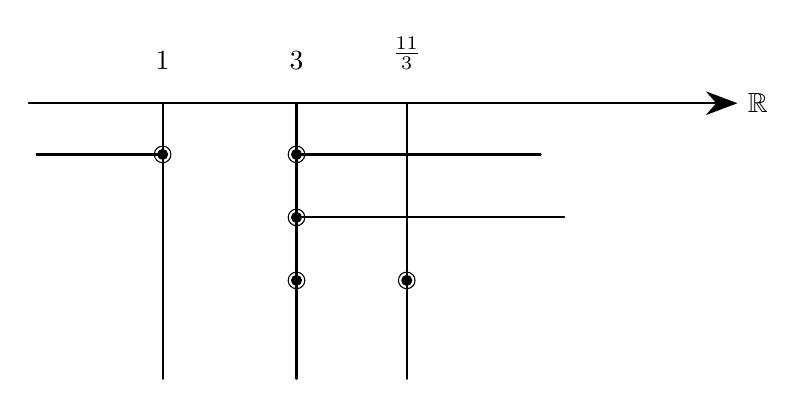
\begin{tikzpicture}[
    line cap=round,
    line join=round
]

% Retta reale orientata
\draw[thick, -{Stealth[length=4mm]}]
    (0,4) -- (9,4)
    node[right] {$\mathbb{R}$};

% Etichette
\node[above=3mm] at (1.7,4) {$1$};
\node[above=3mm] at (3.4,4) {$3$};
\node[above=3mm] at (4.8,4) {$\frac{11}{3}$};

% Linee verticali
\draw[thick] (1.7,4) -- (1.7,0.5);
\draw[thick] (3.4,4) -- (3.4,0.5);
\draw[thick] (4.8,4) -- (4.8,0.5);

% Linee orizzontali: interrotte tra 1 e 3
\draw[thick] (0.1,3.35) -- (1.7,3.35);
\draw[thick] (3.4,3.35) -- (6.5,3.35);
\draw[thick] (3.4,2.55) -- (6.8,2.55);

% Punti
\foreach \x/\y in {
    1.7/3.35,
    3.4/3.35,
    3.4/2.55,
    3.4/1.75,
    4.8/1.75
}{
    \fill (\x,\y) circle (2pt);
    \draw (\x,\y) circle (3pt);
}

\end{tikzpicture}
\end{center}
$$\boxed{x=3\lor x=\frac{11}{3}}$$
\end{exercise}
\begin{exercise}
    $$\sqrt{x+1}=4$$
    $$\begin{cases}
        x+1\ge0&\text{C.E.}\\
        4\ge0&\text{C.S.}\\
        x+1=16
    \end{cases}$$
    $$\begin{cases}
        x\ge1\\
        \forall x\in\mathbb{R}\\
        x=15
    \end{cases}$$
    

\begin{center}
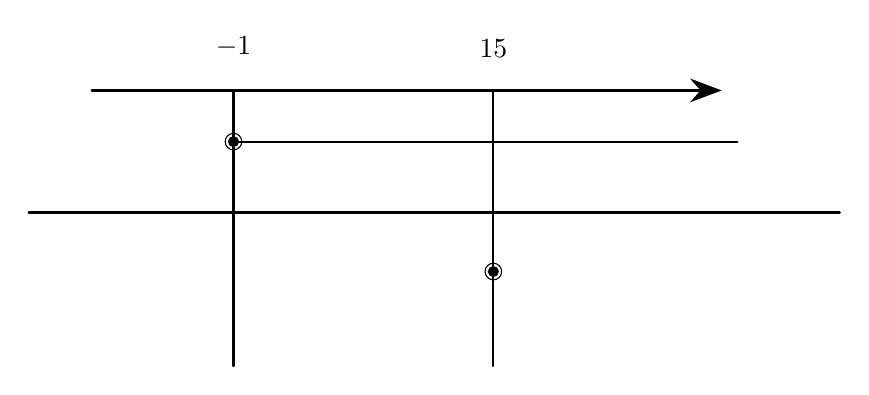
\begin{tikzpicture}[
    line cap=round,
    line join=round
]

% Retta orientata senza etichetta A
\draw[thick, -{Stealth[length=4mm]}]
    (0,4) -- (8,4);

% Etichette
\node[above=3mm] at (1.8,4) {$-1$};
\node[above=3mm] at (5.1,4) {$15$};

% Linee verticali
\draw[thick] (1.8,4) -- (1.8,0.5);
\draw[thick] (5.1,4) -- (5.1,0.5);

% Linee orizzontali
\draw[thick] (1.8,3.35) -- (8.2,3.35);
\draw[thick] (-0.8,2.45) -- (9.5,2.45);

% Punti evidenziati
\fill (1.8,3.35) circle (2pt);
\draw (1.8,3.35) circle (3pt);

\fill (5.1,1.7) circle (2pt);
\draw (5.1,1.7) circle (3pt);

\end{tikzpicture}
\end{center}
$$\boxed{x=15}$$
\end{exercise}
\end{document}
